\chapter{CubeSats y rl entorno de órbita baja terrestre} \label{chap:cubesat_leo}
El presente capítulo describe el marco tecnológico y orbital en el que se inserta el amplificador de potencia diseñado en esta tesina. La primera parte caracteriza al CubeSat como clase de nanosatélite, su origen, su clasificación por unidades y su modo de lanzamiento. La segunda parte describe la órbita terrestre baja (LEO, del inglés Low Earth Orbit), sus condiciones ambientales y las restricciones que impone sobre el subsistema de comunicaciones. Estos dos ejes justifican las especificaciones de potencia, masa y robustez consideradas en el diseño del amplificador Clase AB en banda S presentado en capítulos posteriores.

\section{Origen y clasificación de los CubeSats}
Un CubeSat es un nanosatélite que adopta un factor de forma estandarizado, definido mediante una unidad de volumen denominada U, equivalente a un cubo de 10 cm de arista. El estándar surge como un esfuerzo conjunto entre la California Polytechnic State University y el Space Systems Development Laboratory de Stanford University, con el objetivo de reducir el costo y el tiempo de desarrollo de misiones espaciales universitarias y aumentar el ritmo de lanzamientos de misiones \cite{cubesatspecs}.

La clasificación CubeSat se diferencia de la clasificación general de pequeños satélites, que agrupa a cualquier satélite de masa inferior a 300 kg sin imponer restricciones de forma. Un CubeSat, en cambio, se ve restringido por dimensiones y masas específicas por unidad, resumidas en la Tabla \ref{tab:cubesat_units}. La estandarización habilita la fabricación de componentes de uso general y reduce los costos de integración y de transporte hacia el vehículo lanzador \cite{nasa2017}.

\begin{table}[htbp]
    \centering
    \caption{Configuraciones estandarizadas de CubeSat según la especificación CDS Rev. 14.1 \cite{cubesatspecs}.}
    \label{tab:cubesat_units}
    \begin{tabular}{lcc}
        \hline\hline
        Configuración & Dimensiones nominales (cm) & Masa máxima (kg) \\
        \hline
        1U   & $10 \times 10 \times 11,35$ & 2,00  \\
        1.5U & $10 \times 10 \times 17,02$ & 3,00  \\
        2U   & $10 \times 10 \times 22,70$ & 4,00  \\
        3U   & $10 \times 10 \times 34,05$ & 6,00  \\
        6U   & $10 \times 20 \times 34,05$ & 12,00 \\
        12U  & $20 \times 20 \times 34,05$ & 24,00 \\
        \hline\hline
    \end{tabular}
\end{table}

Cabe señalar que las primeras revisiones de la \textit{Cubesat Design Specification} (CDS) establecían un límite de masa más conservador para el 1U, cercano a 1,33 kg. Actualmente, en la revisión 14.1, dicho límite es de 2,00 kg por unidad para reflejar la disponibilidad de subsistemas comerciales de mayor densidad \cite{cubesatspecs}.

La comparación con satélites convencionales resulta ilustrativa de las ventajas económicas del formato. Mientras un satélite geoestacionario tradicional demanda entre 150 y 350 millones de dólares y entre 5 y 15 años de desarrollo, un CubeSat puede desarrollarse por menos de 200000 dólares en un plazo menor al año. Como contraparte, la vida últil de un cubesat se encuentra en el rango de 2 a 4 años mientras que la de un satélite convencional suele ser de 5 a 15 años \cite{zeedan2023}. 

La reducción de costos y de tiempos de desarrollo explica el crecimiento sostenido de la cantidad de misiones CubeSat lanzadas, así como la diversificación de sus aplicaciones hacia sensado remoto, comunicaciones, navegación satelital, astronomía y exploración interplanetaria. Un relevamiento reciente contabiliza 1523 misiones CubeSat lanzadas entre 2017 y 2024, agrupadas en 26 categorías de misión, entre las cuales las misiones de sensado remoto y de telecomunicaciones concentran la mayor proporción \cite{tubbal2025}. El gráfico de barras de la Figura~\ref{fig:mission_types} muestra la distribución de misiones CubeSat según aplicación.

\begin{figure}[H]
    \centering
    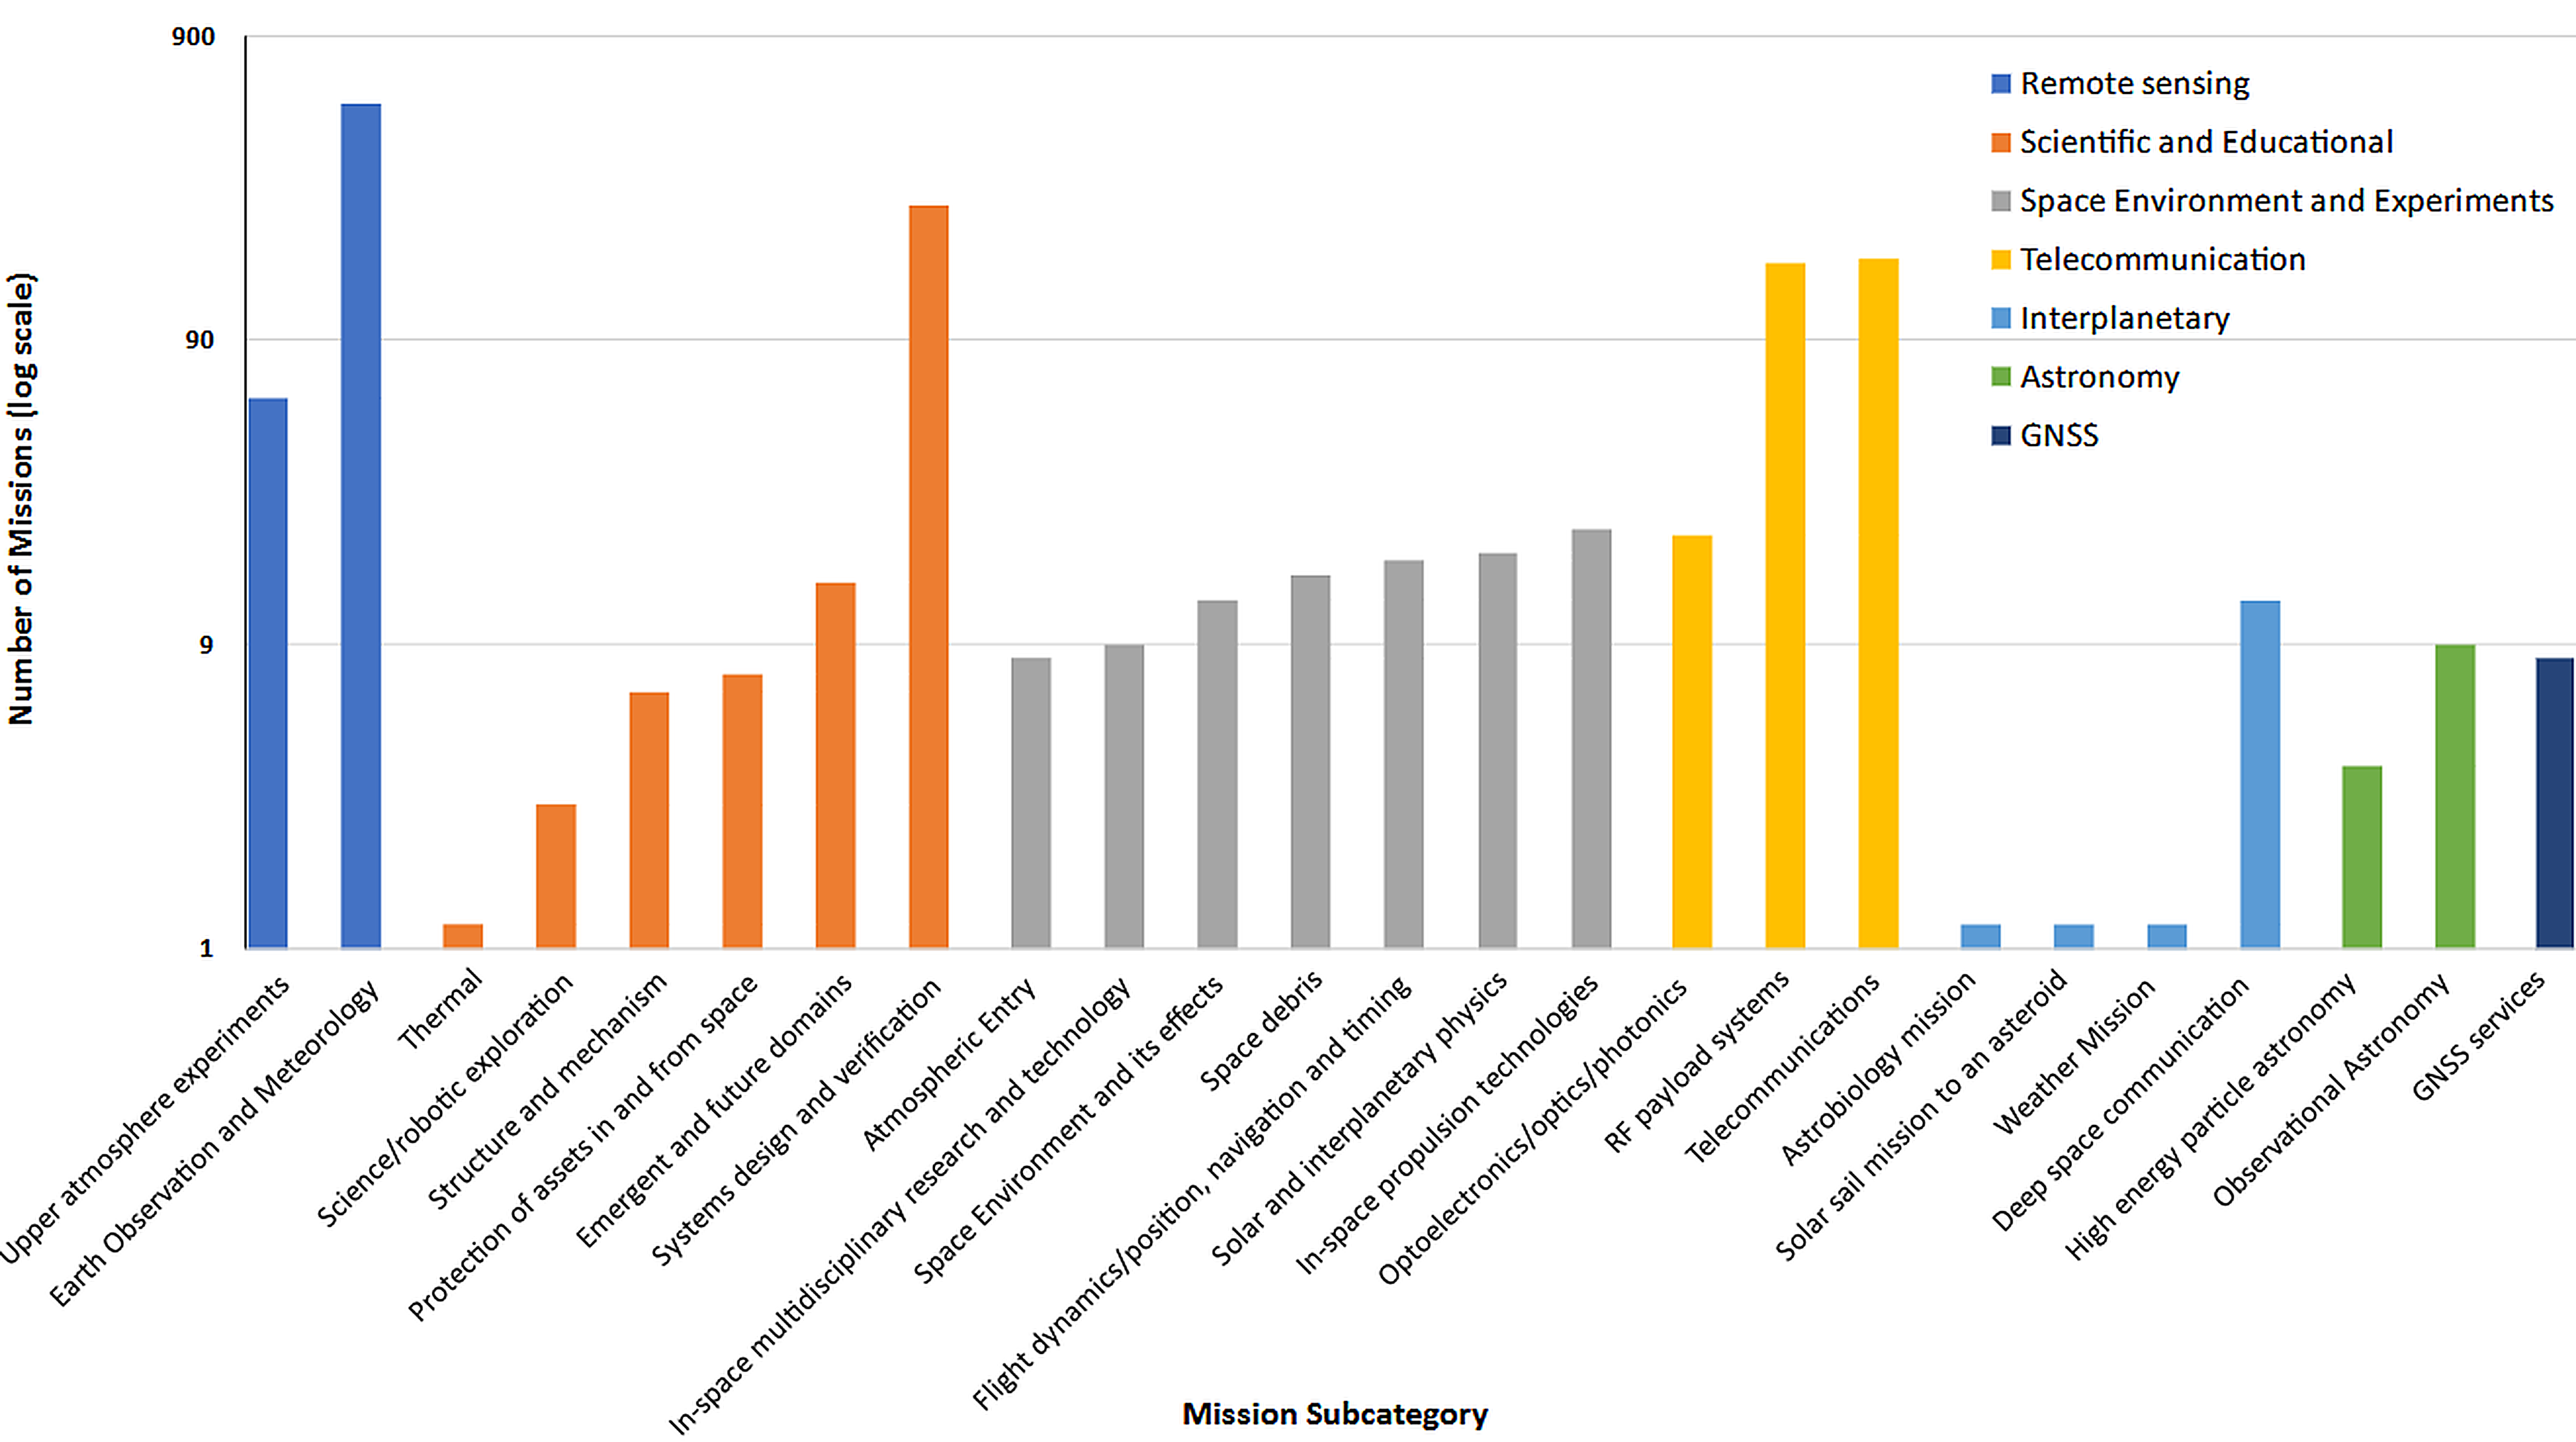
\includegraphics[width=\textwidth]{Figures/cubesat_mission_types_hires.png}
    \caption{Distribución de misiones CubeSat según el tipo de aplicación \cite{tubbal2025}.}
    \label{fig:mission_types}
\end{figure}

El lanzamiento de un CubeSat no se realiza de manera independiente, sino mediante un dispensador que actúa como interfaz mecánica entre el satélite y el vehículo lanzador. El primer dispensador desarrollado con este fin fue el Poly Picosatellite Orbital Deployer (P-POD), capaz de alojar hasta 3U. Un mismo dispensador aloja habitualmente varios CubeSats de distintos desarrolladores en una única posición de lanzamiento, y un mismo vehículo lanzador transporta a su vez varios dispensadores como carga secundaria \cite{cubesatspecs,nasa2017}. Esta modalidad de lanzamiento compartido explica la existencia de constelaciones completas de CubeSats, como las operadas por empresas dedicadas a la observación terrestre \cite{zeedan2023}. Alternativamente, un CubeSat puede desplegarse desde la Estación Espacial Internacional \cite{nasa2017}.

\section{Restricciones del formato CubeSat}
\label{sec:restricciones_cubesat}
El cumplimiento de la especificación CDS condiciona directamente los márgenes disponibles para el subsistema de comunicaciones. Entre las restricciones mecánicas se destaca la masa máxima permitida por unidad indicada en la Tabla \ref{tab:cubesat_units}, con un centro de masa acotado a pocos centímetros del centro geométrico del satélite. Entre las restricciones eléctricas, la especificación exige que el sistema de potencia permanezca completamente apagado hasta la eyección del satélite y que la transmisión de radiofrecuencia no comience antes de los 45 minutos posteriores al despliegue, requisito que obliga a incluir al menos tres inhibidores independientes de transmisión. Asimismo, la especificación fija un límite de energía cinética de reingreso inferior a 15 J por componente, en línea con las directrices de mitigación de basura espacial de la NASA (NPR 8715.6) \cite{cubesatspecs}.

Estas restricciones de masa y de volumen determinan de manera directa el presupuesto de potencia disponible para el subsistema de radiofrecuencia. Dado que la potencia generada por los paneles solares de un CubeSat de reducidas dimensiones resulta limitada, el amplificador de potencia debe alcanzar la potencia de salida especificada con la máxima eficiencia posible.

\section{La órbita terrestre baja (LEO)}
\subsection{Definición y rango altitudinal}
La órbita terrestre baja comprende, en su definición más amplia, las trayectorias satelitales cuya altitud se ubica hasta los 2000 km sobre la superficie terrestre. Dentro de este rango, la densidad espacial de objetos catalogados no resulta uniforme. La Figura \ref{fig:leo_density} muestra la densidad espacial, expresada en objetos por kilómetro cúbico, de objetos desplegados intencionalmente, de basura espacial y del total combinado, en función de la altitud, para el catálogo de objetos rastreados por la Red de Vigilancia Espacial de los Estados Unidos \cite{anzmeador2018}. Se observa una concentración marcada de objetos catalogados en la región comprendida entre los 700 km y los 1000 km de altitud.
 
\begin{figure}[htbp]
    \centering
    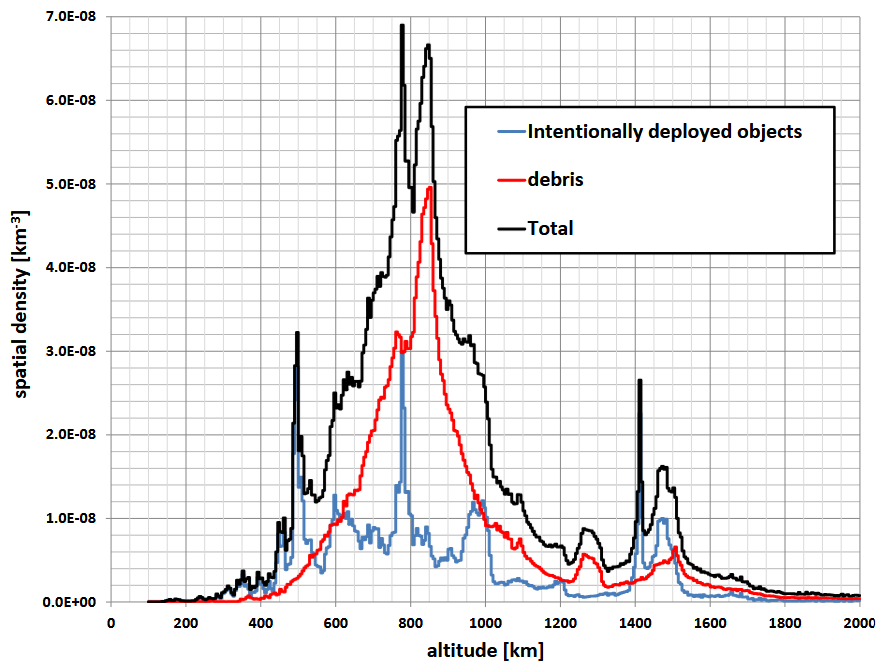
\includegraphics[width=0.85\textwidth]{Figures/leo_population.png}
    \caption{Densidad espacial de objetos catalogados en órbita terrestre baja en función de la altitud \cite{anzmeador2018}.}
    \label{fig:leo_density}
\end{figure}

Las misiones CubeSat, en cambio, tienden a operar en un subconjunto más acotado del rango altitudinal total de LEO. El estudio de presupuestos de enlace de \cite{popescu2017} asume altitudes de misión CubeSat entre 200 km y 800 km, con inclinaciones habituales de 52\textdegree{} para las altitudes menores a 500 km y de 98\textdegree{} (órbita heliosíncrona) para las altitudes superiores, criterio respaldado por el relevamiento de parámetros orbitales de 258 CubeSats registrados por el North American Aerospace Defense Command (NORAD), que confirma que la gran mayoría de las misiones adopta trayectorias circulares, con excentricidad cercana a cero \cite{popescu2017}. Este rango es a su vez consistente con el de la mayoría de las misiones CubeSat relevadas entre 2017 y 2024, cuya altitud de operación se concentra predominantemente entre 400 km y 740 km \cite{tubbal2025}. Resulta relevante notar que las altitudes típicas de operación CubeSat se ubican, en su mayoría, por debajo de la región de máxima densidad de basura espacial ilustrada en la Figura \ref{fig:leo_density}, aunque algunas misiones de mayor duración o de mayor altitud pueden aproximarse a dicha región, donde la probabilidad de colisión con fragmentos catalogados resulta considerablemente mayor.

\subsection{Vacío y ambiente térmico}
La ausencia de atmósfera en LEO elimina el mecanismo de convección como vía de transferencia de calor, de modo que el balance térmico del satélite depende de la radiación solar directa, de la radiación indirecta debido a su reflexión en la Tierra, de la radiación infrarroja terrestre y de la disipación interna \cite{gaite2007}. El paso periódico del satélite por la sombra terrestre, con una cadencia de 90 a 95 minutos por órbita, produce ciclos térmicos abruptos entre la fase iluminada y la fase eclipsada, lo cual exige que la estructura y los componentes electrónicos toleren fluctuaciones térmicas significativas dentro de cada órbita. Esta condición resulta particularmente relevante para el diseño del amplificador de potencia, dado que la variación de temperatura afecta el punto de polarización del transistor GaN HEMT y, en consecuencia, sus parámetros de ganancia y de eficiencia, aspecto retomado en el capítulo dedicado a la tecnología GaN HEMT.

El alto vacío introduce además el fenómeno de desgasificación, el cual consiste en un proceso químico a través del que un material libera espontáneamente las especies gaseosas retenidas en su interior \cite{leybold2022}. Este proceso se acentúa en el vacío, dado que dichas especies gaseosas se encuentran menos ligadas al material que a presión atmosférica \cite{chiggiato2020}. Los gases liberados por desgasificación resultan susceptibles a la ionización, condición que puede generar caminos imprevistos de conducción de corriente frente a campos eléctricos intensos, y pueden además reaccionar químicamente con otros elementos del sistema, degradando su calidad o su rendimiento \cite{mks2024}. Por este motivo, la especificación CDS impone límites cuantitativos de pérdida total de masa (TML) y de material condensable volátil colectado (CVCM) sobre los materiales admitidos en un CubeSat, según se indicó en la Sección \ref{sec:restricciones_cubesat} \cite{cubesatspecs}. Adicionalmente, el alto vacío somete a estrés mecánico a los componentes que emplean encapsulados cerrados no sellados en vacío, condición que debe verificarse durante la selección de componentes comerciales de radiofrecuencia \cite{chiggiato2020}.

\subsection{Atmósfera residual}
Aunque la densidad atmosférica decrece de manera monótona con la altitud \cite{benson2021}, en LEO dicha densidad resulta considerablemente menor a la de la superficie terrestre sin llegar a ser despreciable, y decae de manera marcada dentro del propio rango altitudinal de LEO. A modo de ejemplo, el error de predicción orbital introducido por la incertidumbre en los modelos de densidad atmosférica se reduce entre uno y dos órdenes de magnitud al pasar de 250 km a 550 km de altitud, debido a la menor densidad absoluta presente a mayor altura \cite{ray2022vleo}. La atmósfera residual presenta dos problemas fundamentales para el diseño satelital. Primero la presencia de oxígeno atómico, capaz de erosionar y oxidar los materiales poliméricos y los recubrimientos superficiales expuestos, tanto en superficies externas como en cavidades internas con apertura hacia el entorno espacial \cite{banks2003}. Segundo, la fricción aerodinámica entre el satélite y la atmósfera residual, que disipa energía orbital de forma continua y produce un decaimiento progresivo de la altitud. A modo de ejemplo, para una órbita de 450 km de altitud sujeta a actividad solar intensa, la disminución diaria del semieje mayor por efecto del arrastre atmosférico puede superar los 150 m por día \cite{thomassin2017}. Este efecto resulta más pronunciado cuanto menor es la altitud de la órbita, y exige incorporar un subsistema de control de actitud y órbita (AOCS, por sus siglas en inglés) capaz de compensar dicho decaimiento o de planificar maniobras de mantenimiento orbital \cite{thomassin2017}.

\subsection{Campo magnético terrestre}
El campo magnético terrestre no presenta una distribución uniforme sobre la superficie del planeta, y su intensidad y orientación varían de manera apreciable según la latitud y la longitud consideradas \cite{esa2020}. Esta variabilidad geográfica resulta relevante para todo sensor o actuador cuyo funcionamiento dependa del campo magnético, como los empleados en el subsistema de control de actitud de un satélite \cite{miranda2012}. Por otra parte, el campo magnético terrestre cumple una función de escudo frente a la radiación proveniente del sol, usualmente denominada viento solar, al desviar una fracción sustancial de dichas partículas cargadas mediante la fuerza de Lorentz \cite{nasa2025magnet, epa2025}. La fracción de partículas de alta energía que no resulta desviada queda atrapada en dos regiones denominadas cinturones de Van Allen \cite{nasa2025vanallen}. El cinturón externo está compuesto principalmente por miles de millones de partículas de alta energía de origen solar, mientras que el cinturón interno resulta de la interacción de los rayos cósmicos con la atmósfera terrestre \cite{nasa2025vanallen}. La relevancia de estos cinturones para el ambiente de radiación en LEO se desarrolla en la Sección~\ref{sec:radiacion_leo}.

\subsection{Radiación} \label{sec:radiacion_leo}
El entorno de radiación en LEO combina tres componentes principales. En primer lugar, las partículas cargadas atrapadas en los cinturones de Van Allen descriptos en la subsección anterior, compuestas predominantemente por protones y electrones de alta energía. Segundo, las partículas energéticas solares, compuestas mayoritariamente por protones provenientes de llamaradas solares y en menor proporción por partículas alfa, iones pesados y electrones, cuyo flujo se incrementa de manera considerable durante eventos de actividad solar intensa \cite{mikaelian2001}. Tercero, los rayos cósmicos galácticos, provenientes de fuera del sistema solar, compuestos aproximadamente por un 85\% de protones, un 14\% de partículas alfa y un 1\% de núcleos pesados, con energías del orden de los GeV que les permiten penetrar profundamente en los dispositivos semiconductores \cite{mikaelian2001}.
 
Estos tres componentes producen tres categorías distintas de efectos sobre los dispositivos semiconductores. La primera categoría corresponde a los efectos acumulativos, que degradan el dispositivo de manera gradual. La dosis total ionizante (TID, por sus siglas en inglés) resulta de la energía depositada de forma acumulada por electrones y protones, principalmente provenientes de cinturones de Van Allen y de origen solar. El principal problema que ocasiona este tipo de radiacón es el corrimiento gradual de los parámetros eléctricos de dispositivos semiconductor hasta ocasionar su falla \cite{mikaelian2001}. 

En segundo lugar está el daño por desplazamiento, que resulta de la interacción de protones energéticos con la red cristalina del semiconductor. Estos protones desplazan átomos de su posición natural en el cristal, generando huecos e intersticiales, lo cual va formando cúmulos de defectos capaces de alterar las propiedades eléctricas del dispositivo \cite{mikaelian2001}.
 
La tercera categoría corresponde a los eventos de efecto único (SEE, \textit{Single Event Effects}), producidos por el impacto de una partícula individual de alta energía que deja en su trayecto por el material semiconductor una traza de pares electrón-hueco. A su vez, los SEE pueden clasificarse en destructivos y no destructivos \cite{lauenstein2015}. Entre los SEE no destructivos se encuentra el \textit{Single Event Upset} (SEU), que provoca un cambio no deseado en el estado lógico de un dispositivo digital y que resulta reversible, y \textit{Single Event Transient} (SET), que genera un pulso espurio de tensión o corriente sin alterar de manera permanente el estado del dispositivo. Entre los SEE destructivos se encuentra el \textit{Single Event Latchup} (SEL), en el cual la partícula incidente provoca un cambio de estado lógico irreversible de manera espontánea y que puede derivar en corrientes elevadas capaces de destruir el dispositivo si la alimentación no se interrumpe a tiempo, y \textit{Single Event Burnout} (SEB), donde se genera una corriente de gran magnitud debido a la interacción de la partícula incidente en la región de drain, provocando un efecto avalancha, lo cual destruye el dispositivo. A estos se suma la \textit{Single Event Gate Rupture}(SEGR), asociada a dispositivos MOSFET de potencia donde una partícula altamente energética incide sobre el óxido de gate y provoca la ruptura del mismo, ocasionando un cortocircuito entre el gate y el canal \cite{mikaelian2001}.

\subsection{Basura espacial e interferencia} \label{subsec:basura_espacial}
La creciente cantidad de satélites y de fragmentos no funcionales en órbita constituye un riesgo adicional para la operación de CubeSats en LEO, dado que una colisión con un fragmento de reducidas dimensiones puede ocasionar la pérdida total de la misión \cite{tubbal2025}. Por este motivo, la especificación CDS exige que el diseño mecánico y la selección de materiales del CubeSat cumplan con las directrices de mitigación de basura espacial de la NASA, que limitan la energía cinética de reingreso de cualquier componente y establecen criterios de desorbitado al final de la vida útil \cite{cubesatspecs}. En cuanto a la interferencia radioeléctrica, la concentración histórica de misiones en las bandas VHF, UHF y S incrementa la probabilidad de interferencia entre CubeSats que operan en la misma banda y en órbitas próximas \cite{tubbal2025}. Por otra parte, la migración de misiones hacia las bandas S, X y Ka responde principalmente a la creciente demanda de mayores tasas de datos y a la disponibilidad comercial de circuitos integrados de microondas monolíticos (MMIC) para dichas bandas \cite{zeedan2023}.

\subsection{Bandas de frecuencia y esquemas de modulación}
La selección del esquema de modulación en CubeSats evolucionó de manera consistente con la migración hacia bandas de frecuencia más altas. Las primeras misiones, orientadas a telemetría, seguimiento y control (TT\&C) de baja tasa de datos, emplearon predominantemente modulaciones de envolvente constante y baja complejidad de implementación, tales como FSK (Frequency Shift Keying), AFSK (Audio FSK) y GMSK (Gaussian Minimum Shift Keying), operando en las bandas VHF y UHF \cite{zeedan2023, tubbal2025}. Un relevamiento estadístico sobre 182 CubeSats lanzados entre 2015 y 2018 confirma que GMSK constituye el esquema de modulación más utilizado, seguido por BPSK, FSK, QPSK y AFSK \cite{zeedan2023}. Un relevamiento posterior de misiones CubeSat lanzadas entre 2017 y 2024 confirma esta tendencia y muestra que la prevalencia de cada esquema de modulación varía según la categoría de misión considerada, tal como se ilustra en la Figura \ref{fig:tubbal_modulacion} \cite{tubbal2025}.
 
\begin{figure}[htbp]
    \centering
    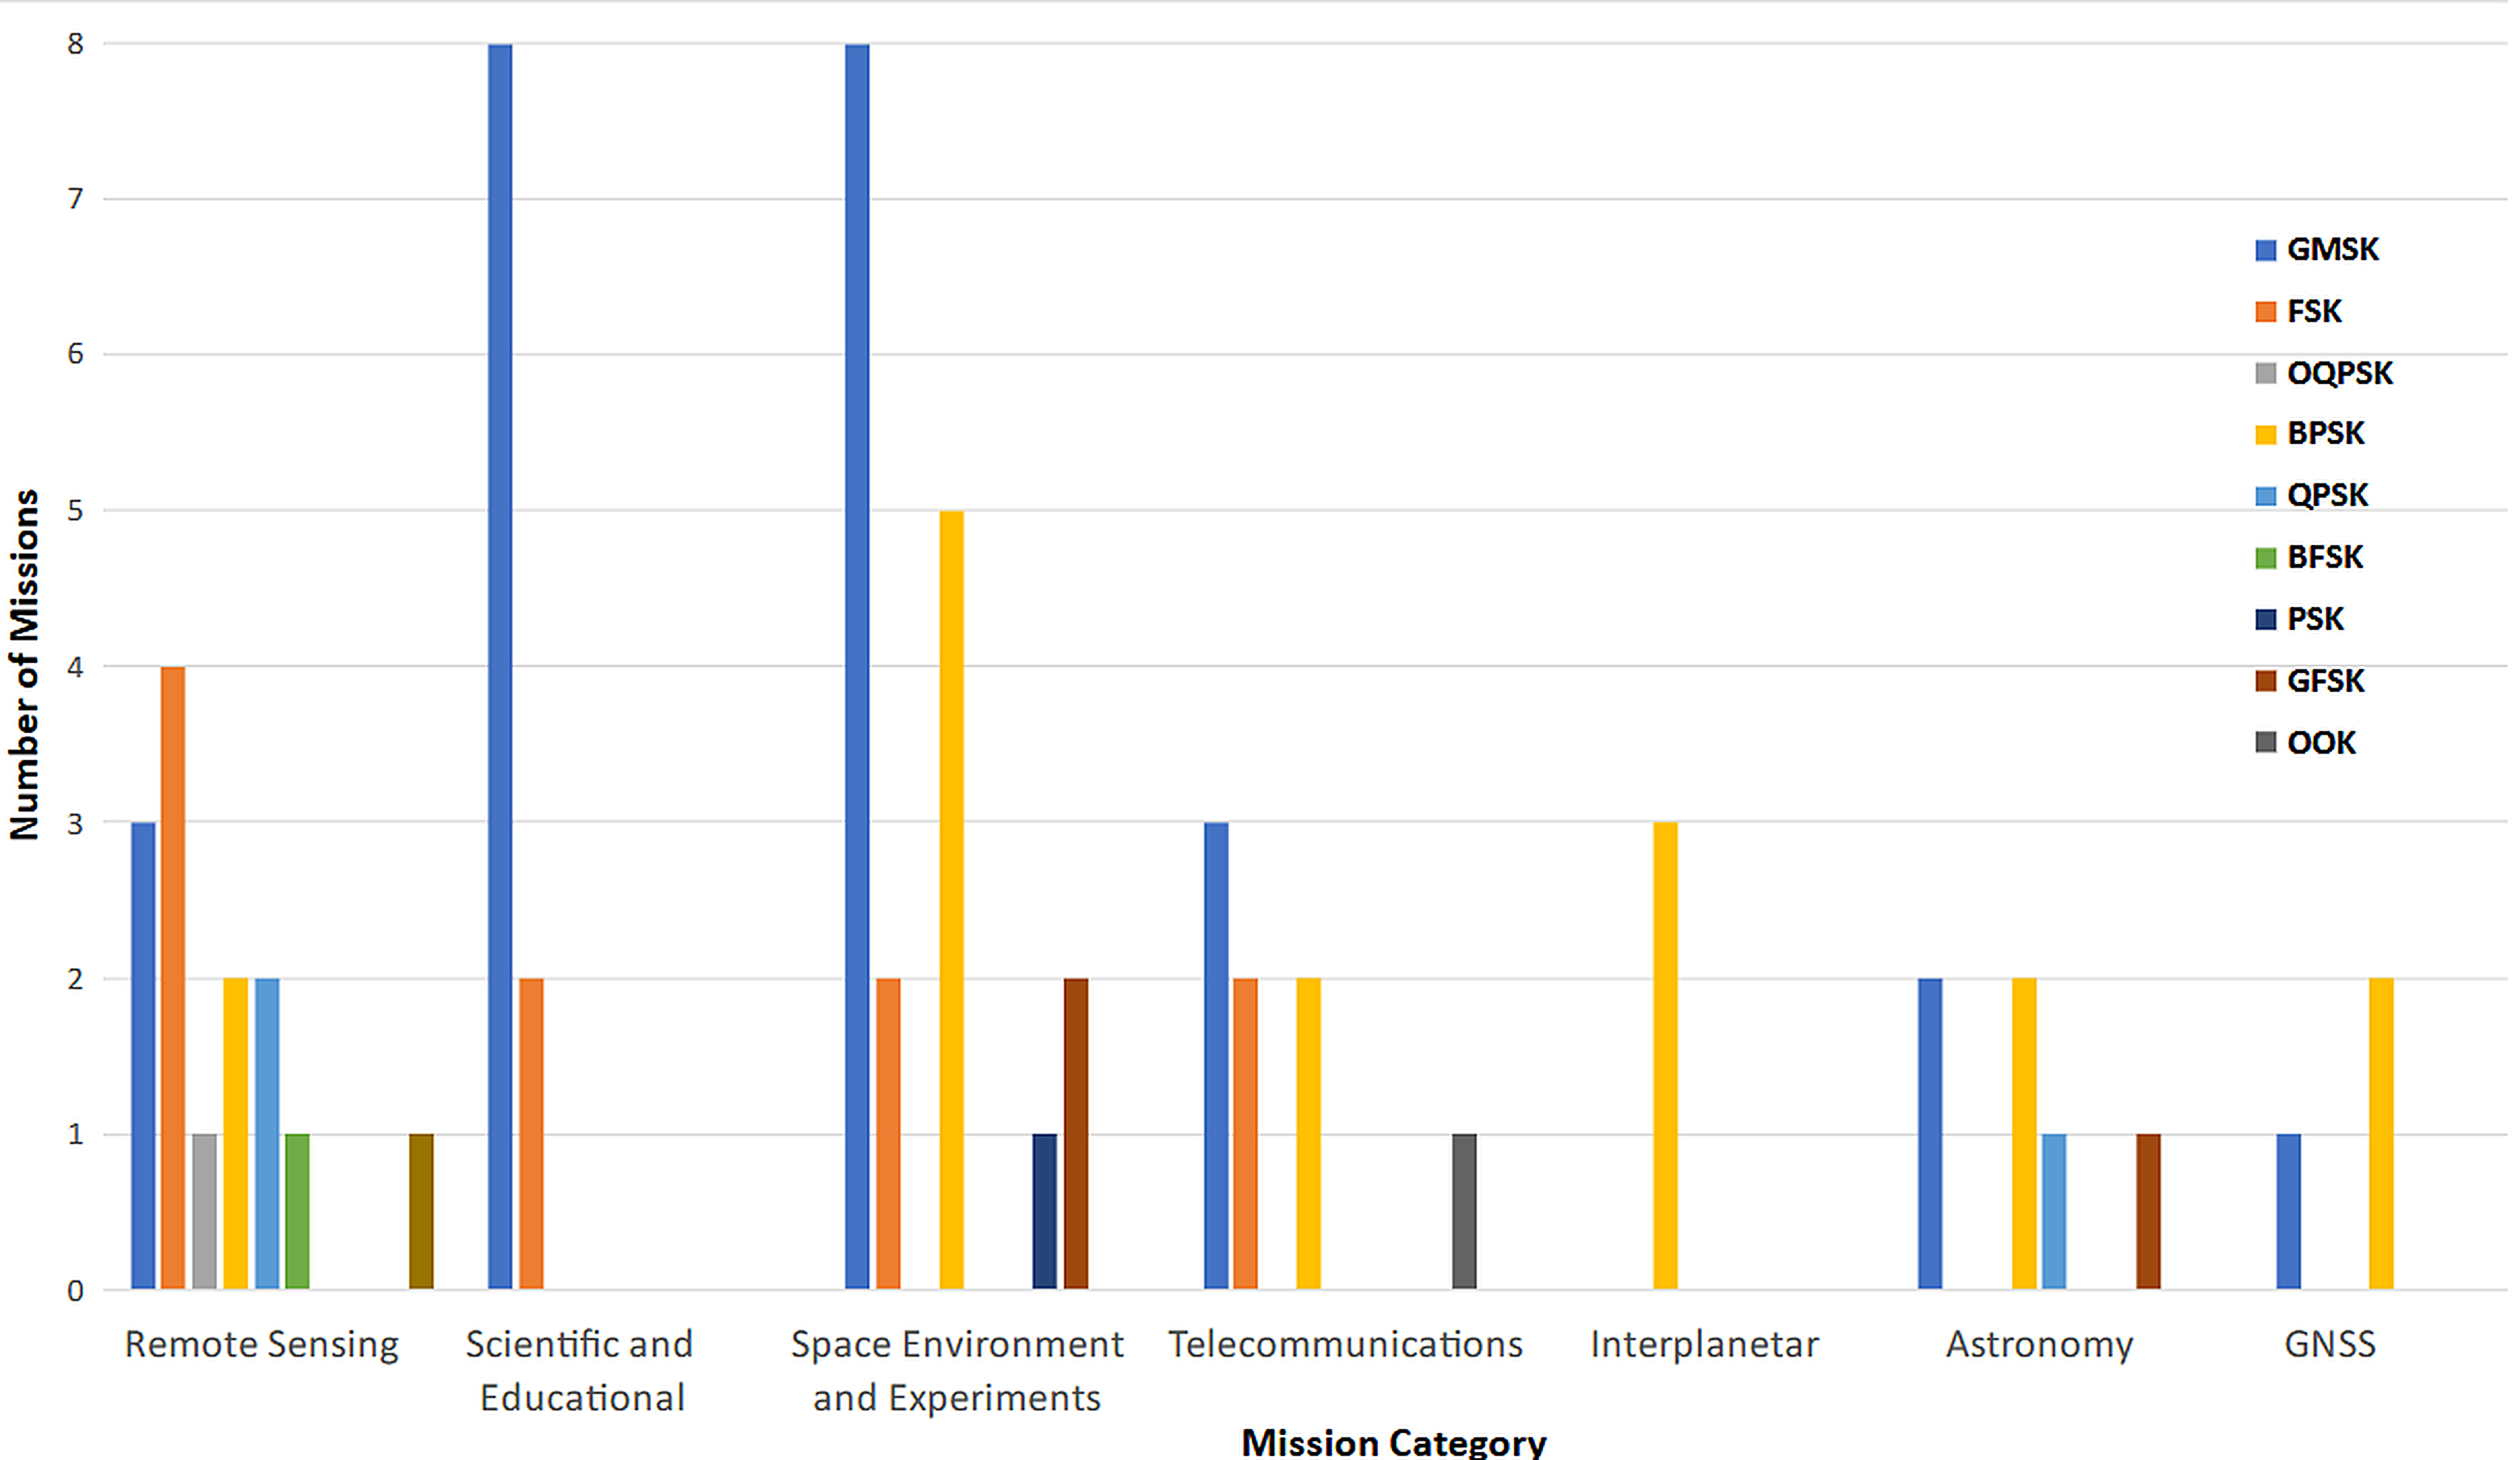
\includegraphics[width=0.95\textwidth]{Figures/modulation_by_mission_hires.png}
    \caption{Distribución de esquemas de modulación empleados en misiones CubeSat, discriminada por categoría de misión. Adaptado de \cite{tubbal2025}.}
    \label{fig:tubbal_modulacion}
\end{figure}
 
A medida que las misiones de sensado remoto y de telecomunicaciones demandaron mayores tasas de datos, la migración hacia las bandas S, X y Ka habilitó el empleo de esquemas de mayor eficiencia espectral, tales como QPSK, 8-PSK, 16-APSK y 32-APSK \cite{zeedan2023, tubbal2025}. Esta migración no resulta uniforme entre categorías de misión: mientras que las operaciones de telemetría, seguimiento y control continúan concentradas mayoritariamente en la banda UHF, los enlaces de carga útil que demandan mayor tasa de datos recurren con mayor frecuencia a las bandas S y X, y las misiones interplanetarias priorizan la banda X por su mayor ganancia de antena a distancias elevadas, según se observa en la Figura~\ref{fig:tubbal_bandas} \cite{tubbal2025}.
 
\begin{figure}[htbp]
    \centering
    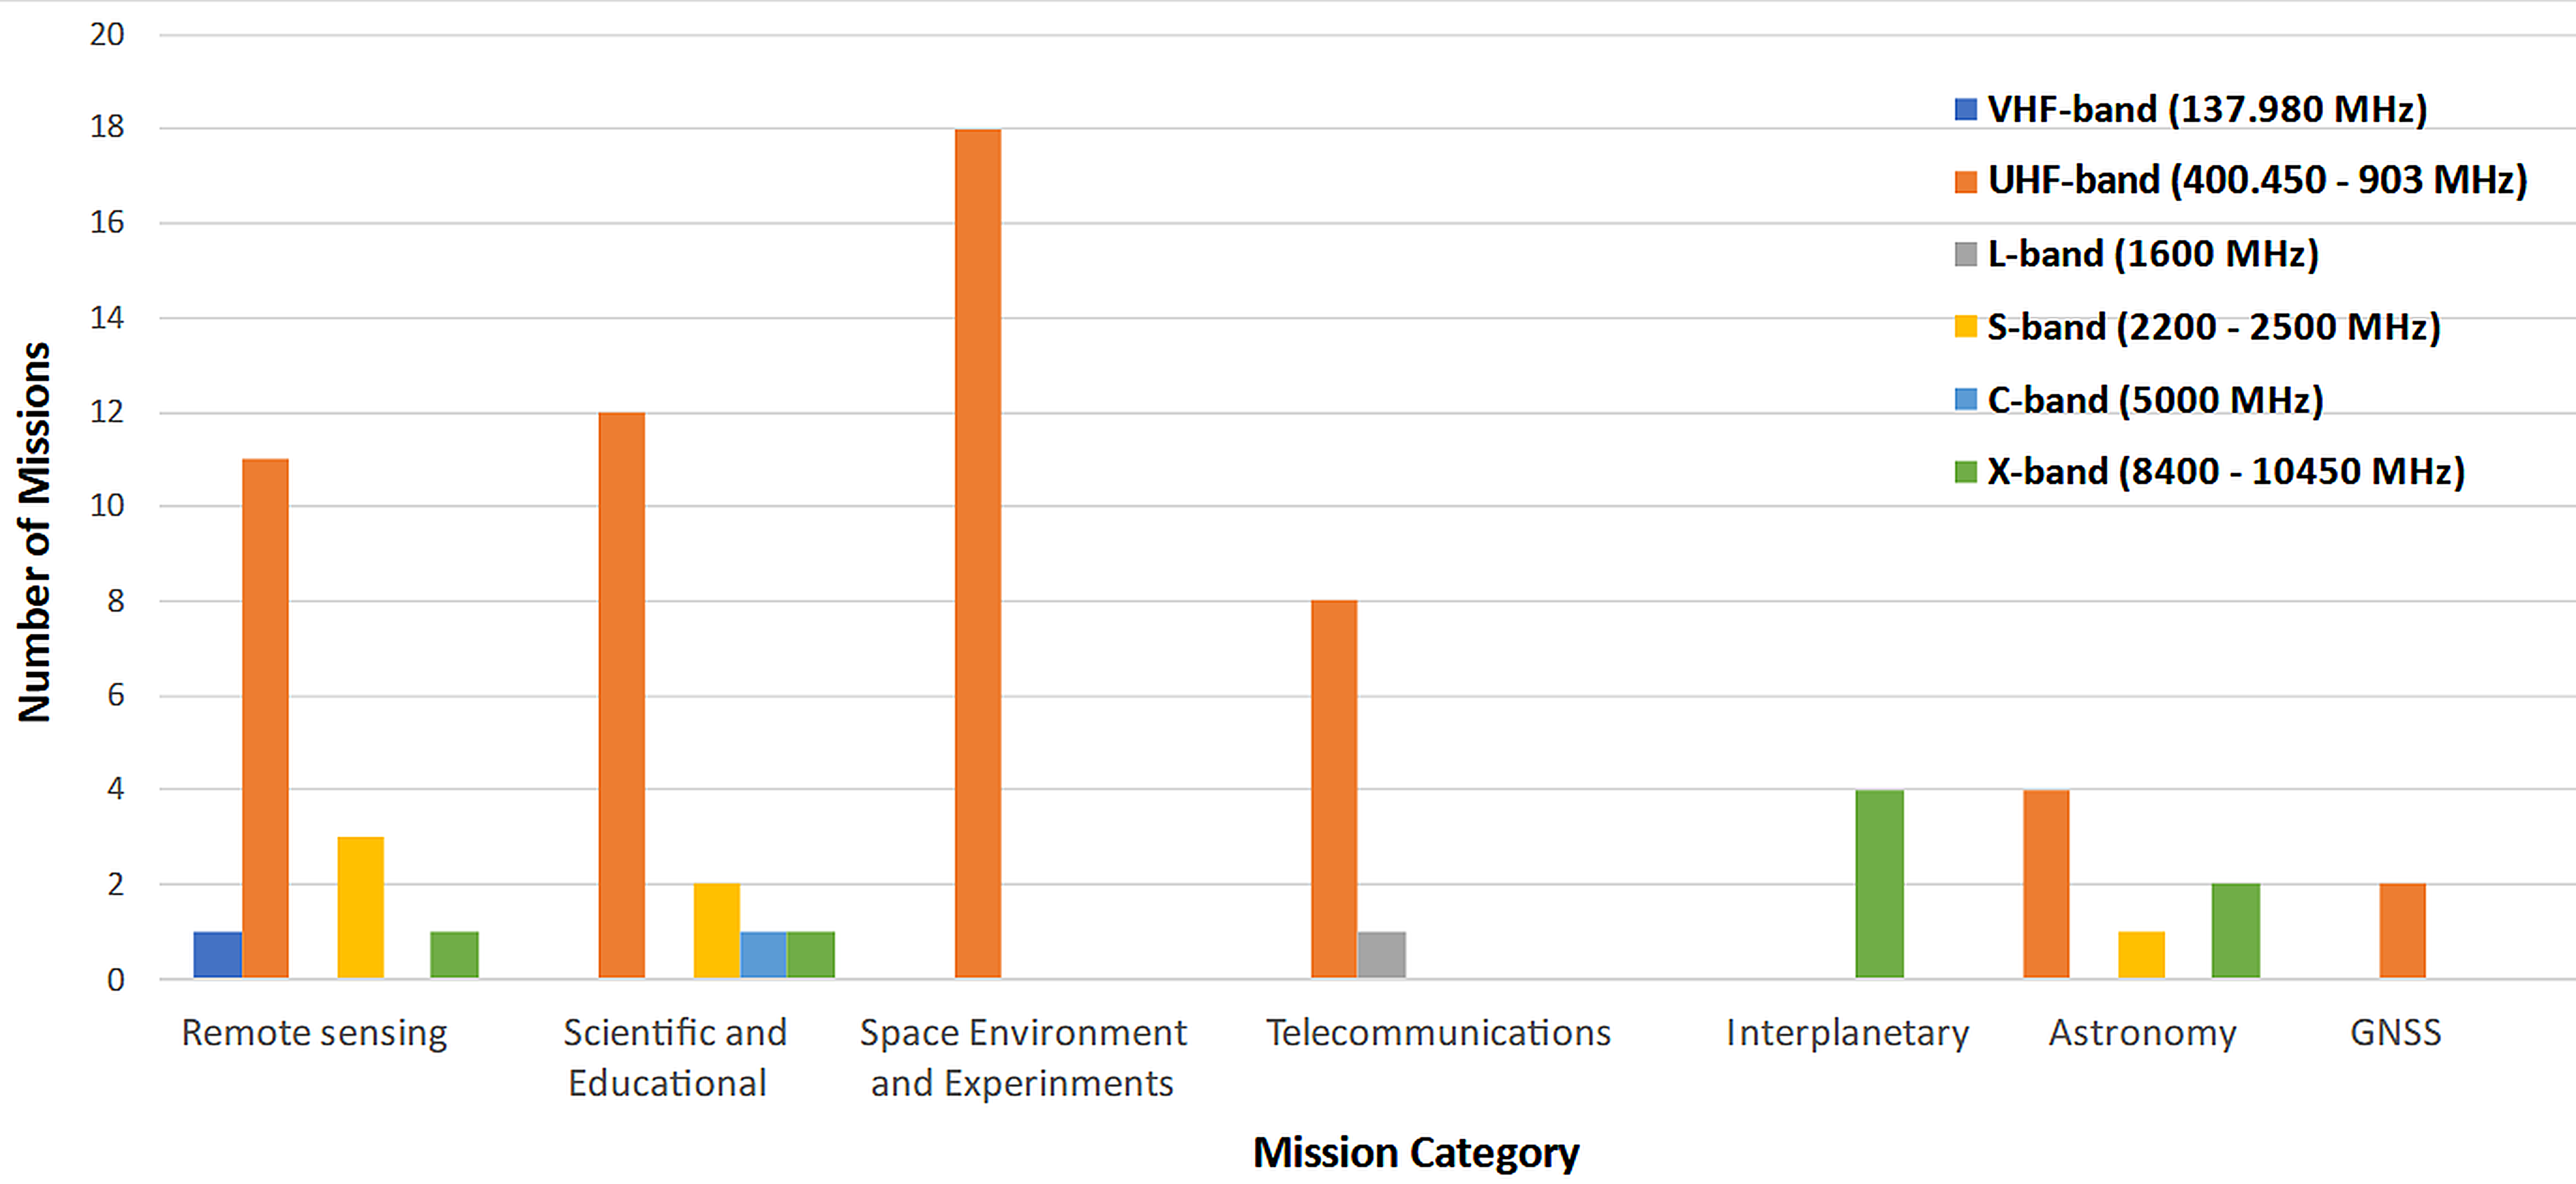
\includegraphics[width=0.95\textwidth]{Figures/freq_by_mission_hires.png}
    \caption{Distribución de bandas de frecuencia empleadas en misiones CubeSat, discriminada por categoría de misión. Adaptado de \cite{tubbal2025}.}
    \label{fig:tubbal_bandas}
\end{figure}
 
La justificación de esta evolución surge de un compromiso entre tres factores. Primero, el ancho de banda ocupado por cada esquema, dado que QPSK y su variante OQPSK (Offset QPSK) requieren un ancho de banda de $8R_b$ para contener el 99\% de la potencia de radiofrecuencia transmitida, frente a $1,2R_b$ para MSK y $0,8R_b$ para GMSK, siendo $R_b$ la tasa de bits \cite{gaysin2017}. Segundo, el desempeño en términos de tasa de error de bit (BER) frente a la relación señal a ruido, en el cual QPSK y OQPSK superan a GMSK para relaciones señal a ruido bajas, mientras que GMSK combinada con demodulación de Viterbi ofrece mejor desempeño a relaciones señal a ruido elevadas, a costa de mayor complejidad computacional y de mayor retardo de demodulación \cite{gaysin2017}. Tercero, la distorsión introducida por la no linealidad del amplificador de potencia, dado que la variante OQPSK evita los saltos de fase de 180\textdegree{} presentes en la modulación QPSK clásica y, en consecuencia, no ocasiona distorsiones profundas en la envolvente de la señal \cite{gaysin2017}. Con base en este compromiso, la literatura especializada en comunicaciones CubeSat propone a QPSK y a OQPSK como los esquemas de modulación de referencia para las misiones CubeSat \cite{gaysin2017}.

\subsection{Duración de las pasadas sobre la estación terrena}
La visibilidad de un CubeSat en LEO desde una estación terrena determinada resulta acotada temporalmente, condición que impone un límite estricto sobre el volumen de datos intercambiable en cada pasada. El período orbital $P$ de un satélite en órbita circular se obtiene a partir de la tercera ley de Kepler, igualando la fuerza gravitatoria a la fuerza centrípeta

\begin{equation}
    \frac{GM_{T}m}{a^{2}} = \frac{4\pi^{2}}{P^{2}}am
    \label{eq:kepler_igualdad}
\end{equation}

donde $G$ es la constante de gravitación universal, $M_{T}$ es la masa terrestre, $m$ es la masa del satélite y $a$ es el semieje mayor de la órbita, que para una órbita circular coincide con la suma del radio terrestre $R_{T}$ y la altitud $H$. Al despejar $P$ de la Ecuación \ref{eq:kepler_igualdad} se obtiene

\begin{equation}
    P = 2\pi\sqrt{\frac{a^{3}}{\mu}}
    \label{eq:periodo_orbital}
\end{equation}

siendo $\mu = GM_{T} \approx 398600,4$ km$^{3}$/s$^{2}$ el parámetro gravitacional terrestre. Para una altitud representativa de misión CubeSat de $H=500$ km, con $R_{T}=6378$ km, el semieje mayor resulta $a=6878$ km. Al reemplazar en la Ecuación \eqref{eq:periodo_orbital} se obtiene $P\approx 5678$ s, equivalente a 94,6 minutos, valor consistente con el período orbital reportado para CubeSats en dicha altitud \cite{popescu2017}.

Sin embargo, el tiempo durante el cual el satélite permanece visible desde una estación terrena determinada, denominado tiempo de pasada, resulta considerablemente menor al período orbital completo, dado que depende adicionalmente de la geometría relativa entre la órbita y la ubicación de la estación terrena, así como de la elevación mínima de horizonte efectivo considerada \cite{popescu2017}. Para una órbita circular de 500 km de altitud e inclinación de 52\textdegree{}, con una estación terrena de referencia, el tiempo de pasada reportado en la literatura varía entre 7,97 minutos, para el caso de una traza que no pasa directamente sobre la estación, y 9,21 minutos, para el caso de máxima elevación \cite{popescu2017}. Este valor, del orden de 5 a 10 minutos, resulta para este ejemplo de diez a doce veces menor al período orbital calculado mediante \eqref{eq:periodo_orbital}.

La brevedad de la ventana de comunicación impone dos consecuencias de diseño directamente vinculadas al amplificador de potencia. Primero, la tasa de datos alcanzable en el enlace descendente, limitada por la potencia disponible en el transmisor del CubeSat, determina el volumen total de información transferible por pasada. A modo de ejemplo, un enlace descendente de 2,4 kbps permite transferir apenas unos 720 kbits durante una pasada corta de 5 minutos \cite{popescu2017}. Segundo, la necesidad de aprovechar íntegramente cada ventana de comunicación exige al amplificador de potencia entregar de manera confiable la potencia de salida especificada desde el instante de activación de la transmisión, sin períodos de estabilización prolongados que reduzcan el tiempo efectivo de enlace.

\section{Síntesis del capítulo}
El formato CubeSat impone restricciones estrictas de masa, de volumen y de potencia disponible, que condicionan de manera directa el presupuesto energético asignable al subsistema de comunicaciones. El entorno de órbita baja terrestre añade a estas restricciones un conjunto de condiciones ambientales exigentes: ciclos térmicos abruptos por la ausencia de convección, desgasificación y estrés mecánico asociados al alto vacío, decaimiento orbital progresivo por atmósfera residual, variabilidad geográfica del campo magnético terrestre, y un régimen de radiación combinado que produce tanto efectos acumulativos (dosis total ionizante y daño por desplazamiento) como eventos de efecto único potencialmente destructivos sobre los dispositivos semiconductores. A esto se suma el riesgo creciente de colisión con basura espacial y la brevedad de las ventanas de comunicación disponibles en cada pasada, del orden de minutos, que limitan de manera estricta el volumen de datos intercambiable con la estación terrena.

El conjunto de estas condiciones fundamenta las decisiones de diseño adoptadas para el amplificador de potencia desarrollado en esta tesina. La robustez del transistor GaN HEMT frente a la radiación acumulada y a los eventos de efecto único, junto con su tolerancia a las fluctuaciones térmicas propias del ciclado orbital, constituyen condiciones necesarias para su empleo en banda S. La elección de una topología Clase AB responde tanto a la necesidad de maximizar la eficiencia dentro del presupuesto de potencia limitado del CubeSat como a la conveniencia de una respuesta rápida que permita aprovechar íntegramente cada ventana de comunicación. Finalmente, la evaluación de esquemas de modulación de envolvente próxima a la constante, tales como QPSK y OQPSK, resulta coherente con la práctica reportada en la literatura de comunicaciones CubeSat y con el compromiso entre linealidad y eficiencia que se desarrolla en el capítulo de teoría del amplificador de potencia.